
\chapter{Tekniske valg}
\newthought {Som en naturlig del av et IT-prosjekt} er de tekniske valgene grunnlaget for prosjektets fundament. I dette kapittelet drøfter vi valg av programmeringsspråk, rammeverk og arkitektur tilhørende denne prosessen.

\section{\textbf{Programmeringsspråk og rammeverk}}
\begin{figure} 
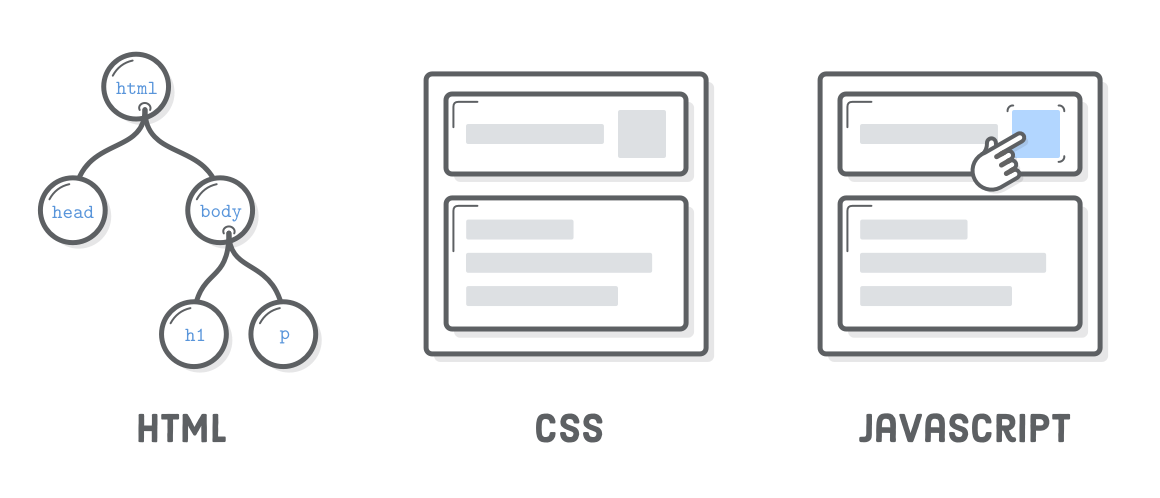
\includegraphics[width=\textwidth]{figures/HTML-CSS-JS.png}
\caption{De tre delene som websider bruker til å samhandle med}
\end{figure}
For å kunne utvikle nettbaserte applikasjoner må man ha kunnskap om HTML, CSS og JavaScript. Denne treenigheten legger grunnlaget for dynamiske, nettbaserte applikasjoner. Tenk på HTML som dokumentet som definerer strukturen til applikasjonen, CSS som den visuelle fremvisningen og JavaScript som definerer applikasjonens dynamiske atferd. 

For å velge et programmeringsspråk og rammeverk som passer prosjektet er det en del kriterier man må drøfte. Blant annet må man ta hensyn til hvilke plattformer man skal utvikle mot, behov for funksjonalitet som ikke støttes universelt og mye mer. I Millum utvikles det primært webapplikasjoner i rammeverkene Angular og React. Vi har vært opptatt av at når vi overleverer prosjektet skal det være så lite hindringer som mulig for videreutvikling. I tillegg er en av de mest sentrale funksjonene i løsningen vår muligheten til å lese strekkoder med mobil og nettbrett. For å ha mulighet til å gjøre dette har vi vært avhengig av å ha tilgang til kameraet på enheten. 

Denne avhengigheten gjør at vi er nødt til å velge et rammeverk som tar i bruk nativefunksjonalitet. I tillegg til å ha mulighet til å bruke nativefunksjonalitet ønsket vi å ha muligheten til å utvikle mot både iOS og Android. Å skulle utvikle to separate løsninger er ikke ideelt da det øker utviklingstiden og behov for vedlikehold dobles. Enkelte utviklingsverktøy lar deg skrive en kodebase og kompilere til forskjellige operativsystemer. Blant disse finner man:

\begin{itemize}
  \item Ionic
  \item React Native, utvikles og oppretholdes av Facebook
  \item Xamarin, Microsoft sitt alternativ
  \item Flutter, Google sitt alternativ
  \item m.m
\end{itemize}

Flere av gruppemedlemmene har erfaring med Angular og React, og muligheten til å velge disse rammeverkene har influert valget. React Native gjør i stor grad utvikleren til å være avhengig av plattformens egne layouter og design, mens Ionic gir utvikler muligheten til å skrive HTML og CSS. Vi har vært opptatte av å følge Millums egne designmanual som følger fargekoder, ikoner og lignende. Det å kunne lett lage egne design og uttrykk fulgte med at vi falt på Ionic med Angular. 

Siden vi har vært opptatt av å følge designmanualen til Millum og i stor grad lage løsningen som en utvidelse av webløsningen har det å lett kunne lage egne design og uttrykk falt valget på Ionic med Angular. 
 
 \subsection{\textbf{Mobilutvikling}}
 For mobilutvikling snakker man ofte om native- og hybrid-utvikling, som er måter å utvikle applikasjonene på. Det å utvikle native gir deg ofte bedre ytelse i store applikasjoner, men gjør i gjengjeld at du må skrive flere separate kodebaser dersom du skal utvikle mot ulike operativsystem. Hybridutvikling er en måte å utvikle mot flere ulike plattformer. Fordelen med å kunne utvikle mot flere plattformer samtidig er at man ofte kan skrive én felles kodebase, men man ofrer gjerne en del av ytelsen som native-utvikling tilbyr deg, samt andre native-funksjoner dersom rammeverket ikke tilbyr dette. 
 
 

\subsection{\textbf{Angular}}
%Hvorfor Angular
Vi valgte Angular som vårt rammeverk fordi det er rammeverket utviklingsteamet til Millum Procurement bruker.  Vår mobilapplikasjon skal være utformet som en en utvidelse av Millum Procurement, og ikke en frittstående applikasjon. Videre vil det å bruke samme rammeverk være hensiktsmessig ettersom Millum selv skal overta prosjektet. Det vil absolutt forenkle prosessene ved videreutvikling og drift for utviklingsteamet.

%Hva er Angular
Angular er et javascript-rammeverk og utviklingsplattform for å utvikle effektive og komplekse Single Page Applications (SPA) i HTML, CSS og TypeScript. TypeScript er et skrevet supersett av JavaScript som kompilerer til vanlig JavaScript. Single Page Applications  betyr kort fortalt at man istedenfor å laste inn hele siden hver gang man navigerer, så laster man kun inn delene av siden som har forandret seg. Dette gjør at innlastingstiden er betydelig lavere enn i en tradisjonell webløsning. 

De fundamentale byggesteinen i Angular er NgModuler, komponenter og tjenestetilbydere. NgModuler er et kjernekonsept i Angular som er en del av enhver applikasjon og hjelper til med å samle viktige detaljer for kompilatoren og applikasjonens driftstid. De er spesielt nyttige for å organisere kode i funksjoner, lazy loading for routing, og lage gjenbrukbare biblioteker. NgModuler kan inneholde komponenter,  tjenestetilbydere og andre kodefiler.

Komponenter definerer hva som vises og inneholder logikk som definerer atferden. Ideelt sett er komponenten sitt ansvar kun selve brukeropplevelsen og ingenting mer. Komponentbasert programvareutvikling vektlegger separasjon av bekymringer med hensyn til den omfattende funksjonaliteten. Selve tankegangen er å skille ut deler av siden til egne komponenter som kan gjenbrukes. 

Tjenestetilbydere, heretter kalt "Service" er en bred kategori som omfatter enhver verdi, funksjon eller funksjon som en app trenger. En service er typisk en klasse med et smalt, veldefinert formål. Den skal gjøre noe spesifikt og gjøre det bra. Vår bruk av services blir utdypet i kapittel \textbf{\ref{kommunikasjon}} 

% Hvordan brukte vi Angular
Vår bruk av Angular er ikke spesielt særegent fra andre Angular-prosjekter. Bruken av NgModuler er noe man må følge etter standard prosedyre, hvis ikke vil applikasjonen ikke kjøre. Derimot er det under bruk av komponenter og servicer man vil se forskjeller fra prosjekt til prosjekt. 


Tankegangen ved komponenter er å ta hvilken som helst nettside og splitt opp i deler av siden. Eksempler på hva som typisk kan være et eget komponent er navigasjonsmenyen, en liste med nyhetsartikler og sidemenyer. Det vil selvsagt variere hvor mange tenkte komponenter man trekker ut etter man har drøftet omfang og kompleksitet for hele applikasjonen.

\subsection{\textbf{Ionic}}

%Hva er Ionic?

Ionic er et open source UI verktøy for å bygge effektive mobil- og web-appklikasjoner veb bruk av tidligere nevnte webteknologier HTML, CSS og JavaScript. Fokuset rammeverket har er på brukeropplevelsen og interaksjon. For hvert Ionic-prosjekt må man også spesifisere hvilket frontend-rammeverk man vil bruke. Ionic tilbyr bruk av Angular, Vue, React og Javascript. Dette samsvarer altså med valg av Angular som rammeverk.

Det Ionic tilbyr oss er ferdige UI komponenter som vi igjen kan velge å tilpasse etter vårt eget designutrykk. Bruken av Ionic sine komponenter er lett å ta i bruk. 

\begin{figure}[H] 
    \centering
    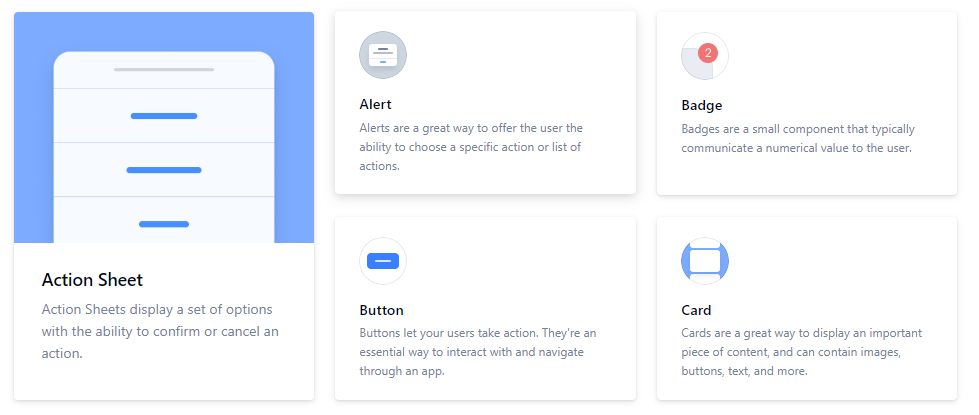
\includegraphics[width=\textwidth]{figures/Tekniske-valg/Ionic/Ionic-Components.PNG}
    \caption{Utsnitt av ferdige komponenter Ionic tilbyr}
\end{figure}

Et eksempel på å legge inn en knapp
\begin{lstlisting}
<ion-button>Ionic knapp!</ion-button>
\end{lstlisting}

%Hva er det i vår applikasjon som kommer fra Ionic rammeverket?

Det er ikke slik at vi kun bruker ferdige Ionic-komponenter, og det er i aller stor grad modifikasjoner på designutrykk der vi velger å bruke deres komponenter. 

\begin{figure}[H] 
    \centering
    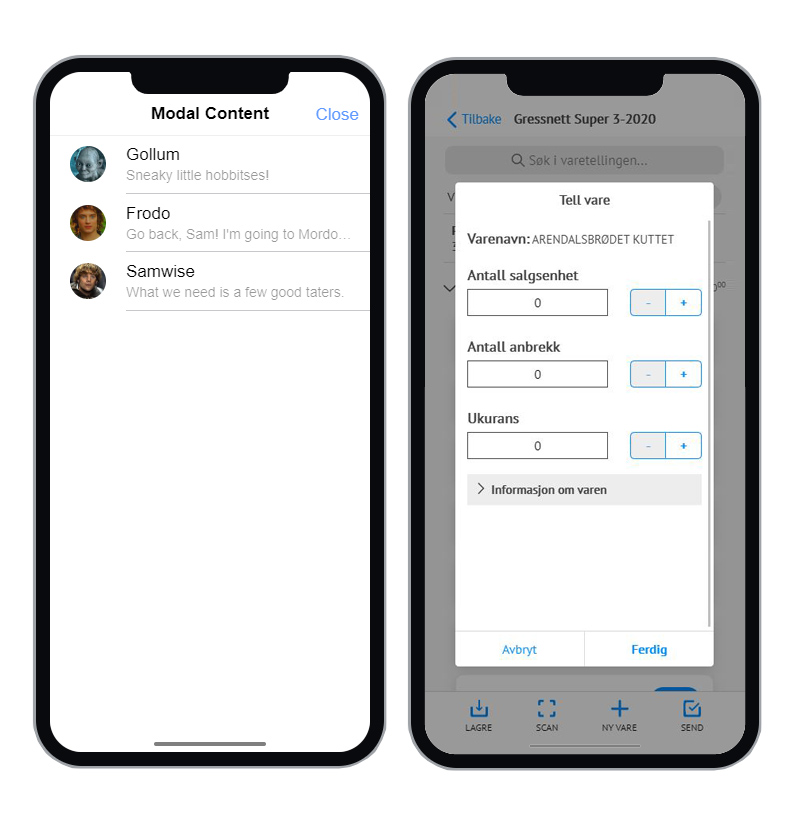
\includegraphics[width=\textwidth]{figures/Tekniske-valg/Ionic/modal.jpg}
    \caption{Ionic sin standard modal-komponent (t.v) sammenlignet med vårt designutrykk (t.h)}
    \label{modalComparison}
\end{figure}

I figuren ovenfor, \textbf{\ref{modalComparison}}, tar vi i bruk en modal, og så stylet det til å ikke ta hele skjermplassen. Dette for å vise brukeren at dette er en funksjonalitet knyttet til siden som vises i bakgrunnen, og at det ikke er en annen side de har navigert seg til.

Ionic tilbyr også native API-løsninger. Native API-løsninger gjør det slik at man kan ta i bruk funksjonalitet som kamerabruk, mobil-tastatur eller fingeravtrykksleser. Det Ionic gjør for oss er i tilgjengeligjøre tilgang til for eksempel kameraet uten at vi må vite de spesifikke detaljene for hvordan iOS eller Android håndterer dette. 


\section{\textbf{Arkitektur}}
Softwarearkitektur refererer til de fundamentale strukturene og disiplinene til å lage et system. Å gjøre gode arkitekturvalg tidlig i prosessen gjør at vi får mulighet til å gjenbruke mest mulig kode og dele sentrale grensesnitt og funksjoner. I dette avsnittet skal vi drøfte arkitekturvalgene våre.

\subsection{\textbf{Kommunikasjon}} \label{kommunikasjon}
I enhver applikasjon er det viktig å definere hvordan kommunikasjonen skal foregå for å gjøre datafangst. I dette avsnittet går vi litt mer i dybden på hvordan kommunikasjonen foregår mellom mobilapplikasjonen og Millum sine API-er.

I løsningen vår er hver datastruktur eller tjeneste (varetelling, produkt osv.) delt inn i egne services. En service er ansvarlig for å tilgjengeliggjøre data når brukeren ber om det. Det kan være i form av at man ønsker å hente data relatert til en varetelling eller et produkt, eller at man ønsker å sende inn sin varetelling.

Servicen som er ansvarlig for å håndtere dette gjør et kall videre til en datatjeneste, heretter kalt “data service”. Data servicen er ansvarlig for selve kommunikasjonen mot API-ene. Kommunikasjonen foregår via Millum sin “Gateway” som igjen er ansvarlig for å lede kommunikasjonen til deres interne tjenester. Resultatet av handlingen data servicen ba om blir levert i en HTTP statuskode. Normalt sett hvis handlingen var vellykket får vi tilbake en statuskode “200”. HTTP-protokollen er en godt utprøvd protokoll for kommunikasjon og blir brukt i de aller fleste webapplikasjoner. All kommunikasjon vi gjør over HTTP-protokollen blir gjort via JSON-format, som er en måte å strukturere dataobjekter på.

Avtalen med Millum er at de leverer API-ene, og vi konsumerer disse igjen i applikasjonen. Dette er et bevisst valg med tanke på sikkerhet, men også med tanke på kompleksiteten og scopet til prosjektet vårt. 

\begin{figure}[H] 
    \centering
    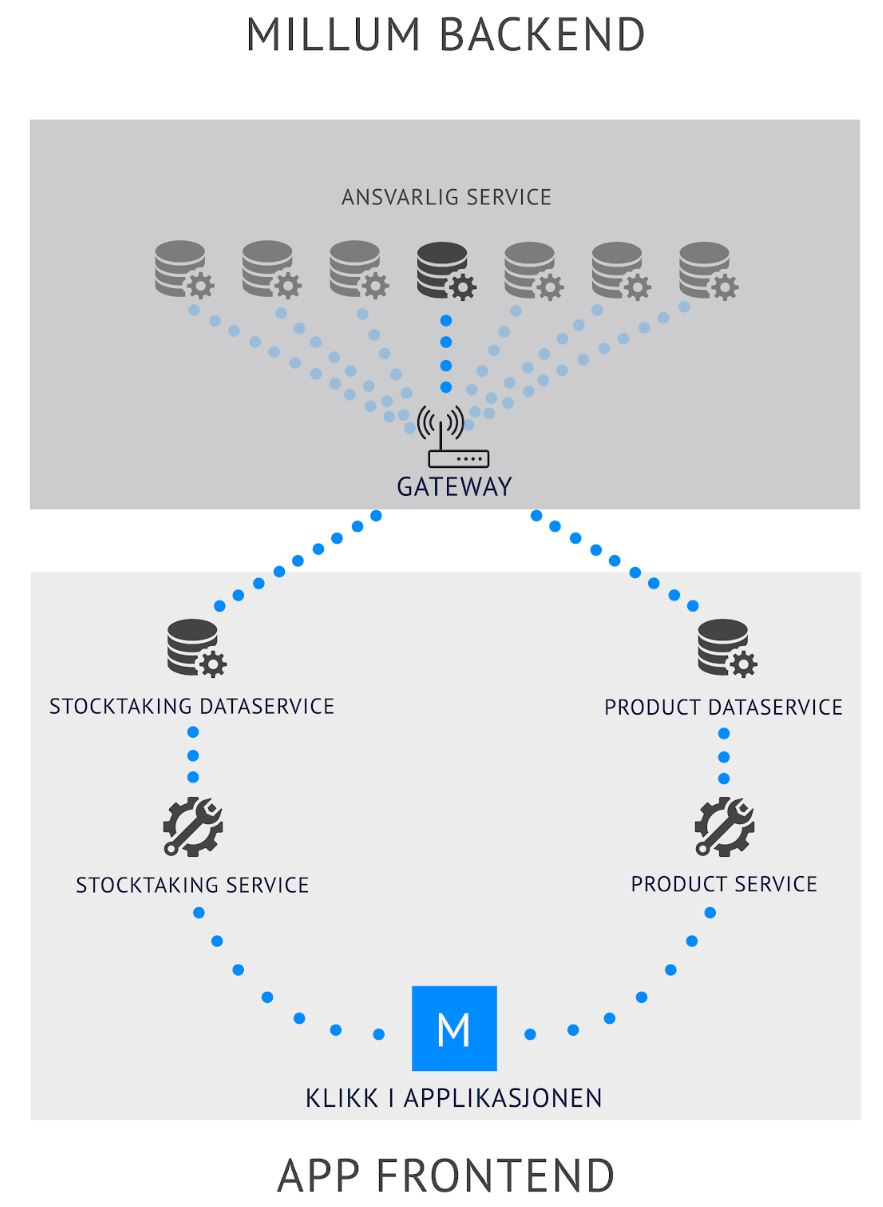
\includegraphics[width=\textwidth]{figures/Tekniske-valg/Arkitektur/kommunikasjon.JPG}
    \caption{Kommunikasjon mellom frontend og backend}
\end{figure}

\subsection{\textbf{Designmønster}}

I årevis har designmønsteret blitt brukt, men det har ikke alltid vært slik at man har vært bevisst på det. Det var arkitekten Christopher Alexander som i 1970-årene konkretiserte konseptet designmønstre innenfor arkitektur-konsepter \cite{christopheralexander}. Videre prøvde man å bruke disse konseptene innenfor programvare-utvikling. Det var derimot ikke før en av de mest kjente bøkene om designmønster,   
Design Patterns: Elements of Reusable Object-Oriented Software, kom på banen i 1994 at utviklere virkelig sperret øynene opp. 


\begin{table}[htbp]
  \centering
  \caption{De fire elementene som beskriver et designmønster \cite{gamma1995design} }
    \begin{tabular}{|l|l|}
\hline
Navnet        & \begin{tabular}[c]{@{}l@{}}Som sier oss noe om design-problemet,\\ løsningen og konsekvensene i ett til to ord\end{tabular} \\ \hline
Problemet     & \begin{tabular}[c]{@{}l@{}}Beskriver når man kan ta i bruk mønsteret\\  og i hvilken kontekst\end{tabular}                  \\ \hline
Løsnigen      & \begin{tabular}[c]{@{}l@{}}Beskrivere elementene som utgjør designet, \\ deres relasjoner, ansvar og samarbeid\end{tabular} \\ \hline
Konsekvensene & \begin{tabular}[c]{@{}l@{}}Beskriver resultatene og avveiningene\\  ved å bruke mønsteret.\end{tabular}                     \\ \hline
\end{tabular}
  \label{tab:addlabel}%
\end{table}%

Design Patterns-boken beskriver flere forskjellige mønstre, og videre går vi dypere inn i hva de forskjellige designmønstrene virker inn i applikasjons-strukturen.

\subsection{\textbf{Model View Controller}}
Model View Controller, MVC,  er et design pattern som deler inn programmet i tre sammenhengende elementer.

\begin{description}
  \item[$\bullet$ Model:] Beskriver programmets struktur uavhengig av grensesnittet. Modellen håndterer og bestemmer reglene og logikken til programmet.
  \item[$\bullet$ View:] Grensesnittet til programmet. Kan eksempelvis være en side eller et diagram.
  \item[$\bullet$ Controller:] Tar i mot hendelser fra viewet og interagerer med modellen.
\end{description}

To store fordeler med MVC er

1. Du kan ha flere views knyttet til én modell for å gi forskjellige presentasjoner av samme data.

2. Endre viewet til å respondere på brukerinnspill uten å endre den visuelle representasjonen

 I vår løsning har vi hatt ansvar for å lage modellen og viewet, mens controlleren kommuniserer med oppdragsgiver egne tjenester. Et eksempel på hvordan dette henger sammen er at brukeren logger inn og skal hente sine varetellinger. Dette gjøres via et API-request til varetellingscontrolleren, som leverer tilbake informasjon som modellen strukturerer og videre presenteres i viewet. 

\subsection{\textbf{Rule of One og Single Responsibility}}
Single responsibility-prinsippet ble først introdusert av Robert C.Martin i hans artikkel med samme navn som en del av Principles of Object Oriented Design, gjort populært av hans bok Agile Software Development, Principles, Patterns, and Practices. Martin definerer responsibility i sin bok Agile Pratices, Patterns and Pratices in C\# som “In the context of the SRP, we define a responsibility to be a reason for change.” (Side 158). Definisjonen er noe tvetydig i formuleringen “a reason for change”. Martin fordyper denne definisjonen i et blogginnlegg kalt The Single Responsibility Principle.  

Rule of One bygger på et annet prinsipp kalt single responsibility. Kort beskrevet kan man si at alle komponenter, servicer og andre symboler kun skal gjøre én ting. Hensikten med dette er å gjøre filen lettere å lese, vedlikeholde og mer gjenbrukbar. I tillegg gjør det at koden er mer testbar, mindre utsatt for bugs og mindre avhengig av annen kode (også kjent som low coupling)

\subsection{\textbf{LIFT}}

\textit{"\textbf{Do} structure the app such that you can \textbf{L}ocate code quickly, \textbf{I}dentify the code at a glance, keep the \textbf{F}lattest structure you can, and \textbf{T}ry to be DRY"} 

Dette prinsippet skal hjelpe deg som utvikler å finne fram til kode raskt. Vi har valgt å følge LIFT-prinsippet på grunnlag av spørsmålet

\textit{Hvor raskt kan du åpne og jobbe i alle filene du trenger for å lage en funksjon? }

\textbf{Locate} gjør lokalsering av kode intuitivt og raskt. Det vil si å holde relaterte filer nær hverandre. Hvorfor gjør man dette? For å jobbe effektivkt må du kunne lokalisere filer raskt, spesielt npr du ikke kjenner, eller husker, filnavnene. Å holde relaterte filer nør hverandre på et intuitivt sted sparer tid. En beskrivende mappestruktur gjør all verdens forskjell for deg og menneskene som kommer etter deg.

\textbf{Identify} betyr det å ha et beskrivende navn for filene slik at du umiddelbart vet hva filen inneholder og representerer. Her er det viktigere å være beskrivende med filnavnet og holde innholdet i filen kun relatert til navngivningen. Det vil si at man ønsker i aller sterkeste grad følger single responsibilty-prinsippet.

\textbf{Flat} omhandler selve mappestrukturen for prosjektet. Det å ha en flat mappestruktur betyr at man ønsker at en mappe skal maksimalt inneholde syv filer, og heller velge å lage undermapper om man overstiger antall filer. 

På den annen side mener psykologer at mennesker begynner å slite når antallet nærliggende interessante ting overstiger ni \cite{miller1956magical}. 
Så når en mappe har ti eller flere filer, kan det være på tide å lage undermapper. Baser avgjørelsen din på ditt komfortnivå. Bruk en flatere struktur til det er en åpenbar verdi å lage en ny mappe

\textbf{Try to be Dry}, altså ikke repeter deg selv. For eksempel gir det ikke noe mening å lage en fil hetende "stock-taking-list-view.component.html". Dette er en HTML-fil og HTML-filer beskriver jo kun det som vises. Det vil dermed bli repetisjon at filnavnet skal inneholdet ordet "view". Om det derimot er tilfeller hvor noe ikke er åpenbart eller avvikende, så for all del stav det ut.
